%!TEX program = xelatex

\documentclass[11pt,titlepage]{report}
%!TEX root = main.tex

\usepackage[T1]{fontenc}
\usepackage{lmodern}
\usepackage[svgnames]{xcolor}
\usepackage{fontspec} % XeLaTeX required!
\usepackage{graphicx}
\usepackage{circuitikz}
\usepackage{tikz}
\usepackage{pifont}
\usepackage[some]{background}
\usepackage{xltxtra} 
\usepackage{setspace}
\usepackage[absolute]{textpos}
\usepackage[latin1]{inputenc}
\usepackage[english]{babel}
\usepackage{graphicx}
\usepackage{wrapfig}
\usepackage{fullpage}
\usepackage[margin=1in]{geometry}
\usepackage{float}
\usepackage{url}
\usepackage{multicol}
\usepackage{hyperref}
\usepackage{titlepic}
\usepackage{standalone}
\usepackage{siunitx}
\usepackage{booktabs}
\usepackage{amsmath}
\usepackage{unicode-math}
\usepackage{verbatim}
\usepackage{enumitem}
\usepackage{listings}
\usepackage{multirow}
\usepackage{pgfplots}
\pgfplotsset{compat=1.8}
\usepackage{caption} 
\usepackage[parfill]{parskip}
\usepackage{import}
\usepackage[backend=bibtexu,texencoding=utf8,bibencoding=utf8,style=ieee,sortlocale=en_GB,language=auto]{biblatex}
\usepackage[strict,autostyle]{csquotes}
\usepackage[final]{pdfpages}
\usepackage{subcaption}
\usepackage{ifplatform}
%\captionsetup[table]{skip=10pt}


% Fix for includepdf bug in Mac OS X
\newcommand{\insertpdfpath}[1]{
	\ifwindows
	\newcommand{\insertpdf}[2]{\includepdf[pages=##1]{##2}}
	\else
	\newcommand{\insertpdf}[2]{\includepdf[pages=##1]{#1/##2}}
	\fi
}

%set fonts
\setmainfont[Ligatures=TeX]{Myriad Pro}
\setmathfont{Asana Math}
\setmonofont{Lucida Console}

\usepackage{titlesec, color}
\renewcommand{\familydefault}{\sfdefault} %set font family
\renewcommand{\arraystretch}{1.2} %set table vertical spacing
\setlength\parindent{0pt} %no paragraph indent
\hypersetup{ %setup hyperlinks
    colorlinks,
    citecolor=black,
    filecolor=black,
    linkcolor=black,
    urlcolor=black
}

%redesign chapter headings
\definecolor{gray75}{gray}{0.75}
\newcommand{\chapternumber}{\thechapter}
\newcommand{\hsp}{\hspace{20pt}}
\titleformat{\chapter}[hang]{\Huge\bfseries}{\chapternumber\hsp\textcolor{gray75}{|}\hsp}{0pt}{\Huge\bfseries}

%Redefine appendix headers
\renewcommand{\appendixname}{Appendix}
\renewcommand{\appendixtocname}{Appendices}
\renewcommand{\appendixpagename}{Appendices}

%For code listings
\definecolor{black}{rgb}{0,0,0}
\definecolor{browntags}{rgb}{0.65,0.1,0.1}
\definecolor{bluestrings}{rgb}{0,0,1}
\definecolor{graycomments}{rgb}{0.4,0.4,0.4}
\definecolor{redkeywords}{rgb}{1,0,0}
\definecolor{bluekeywords}{rgb}{0.13,0.13,0.8}
\definecolor{greencomments}{rgb}{0,0.5,0}
\definecolor{redstrings}{rgb}{0.9,0,0}
\definecolor{purpleidentifiers}{rgb}{0.01,0,0.01}


\lstdefinestyle{csharp}{
language=[Sharp]C,
showspaces=false,
showtabs=false,
breaklines=true,
showstringspaces=false,
breakatwhitespace=true,
escapeinside={(*@}{@*)},
columns=fullflexible,
commentstyle=\color{greencomments},
keywordstyle=\color{bluekeywords}\bfseries,
stringstyle=\color{redstrings},
identifierstyle=\color{purpleidentifiers},
basicstyle=\ttfamily\small}

\lstdefinestyle{c}{
language=C,
showspaces=false,
showtabs=false,
breaklines=true,
showstringspaces=false,
breakatwhitespace=true,
escapeinside={(*@}{@*)},
columns=fullflexible,
commentstyle=\color{greencomments},
keywordstyle=\color{bluekeywords}\bfseries,
stringstyle=\color{redstrings},
identifierstyle=\color{purpleidentifiers},
}

\lstdefinestyle{matlab}{
language=Matlab,
showspaces=false,
showtabs=false,
breaklines=true,
showstringspaces=false,
breakatwhitespace=true,
escapeinside={(*@}{@*)},
columns=fullflexible,
commentstyle=\color{greencomments},
keywordstyle=\color{bluekeywords}\bfseries,
stringstyle=\color{redstrings},
identifierstyle=\color{purpleidentifiers}
}

\lstdefinestyle{vhdl}{
language=VHDL,
showspaces=false,
showtabs=false,
breaklines=true,
showstringspaces=false,
breakatwhitespace=true,
escapeinside={(*@}{@*)},
columns=fullflexible,
commentstyle=\color{greencomments},
keywordstyle=\color{bluekeywords}\bfseries,
stringstyle=\color{redstrings},
identifierstyle=\color{purpleidentifiers}
}

\lstdefinestyle{xaml}{
language=XML,
showspaces=false,
showtabs=false,
breaklines=true,
showstringspaces=false,
breakatwhitespace=true,
escapeinside={(*@}{@*)},
columns=fullflexible,
commentstyle=\color{greencomments},
keywordstyle=\color{redkeywords},
stringstyle=\color{bluestrings},
tagstyle=\color{browntags},
morestring=[b]",
  morecomment=[s]{<?}{?>},
  morekeywords={xmlns,version,typex:AsyncRecords,x:Arguments,x:Boolean,x:Byte,x:Char,x:Class,x:ClassAttributes,x:ClassModifier,x:Code,x:ConnectionId,x:Decimal,x:Double,x:FactoryMethod,x:FieldModifier,x:Int16,x:Int32,x:Int64,x:Key,x:Members,x:Name,x:Object,x:Property,x:Shared,x:Single,x:String,x:Subclass,x:SynchronousMode,x:TimeSpan,x:TypeArguments,x:Uid,x:Uri,x:XData,Grid.Column,Grid.ColumnSpan,Click,ClipToBounds,Content,DropDownOpened,FontSize,Foreground,Header,Height,HorizontalAlignment,HorizontalContentAlignment,IsCancel,IsDefault,IsEnabled,IsSelected,Margin,MinHeight,MinWidth,Padding,SnapsToDevicePixels,Target,TextWrapping,Title,VerticalAlignment,VerticalContentAlignment,Width,WindowStartupLocation,Binding,Mode,OneWay,xmlns:x}
}

\lstdefinestyle{matlab}{
language=Matlab,
showspaces=false,
showtabs=false,
breaklines=true,
showstringspaces=false,
breakatwhitespace=true,
escapeinside={(*@}{@*)},
columns=fullflexible,
commentstyle=\color{greencomments},
keywordstyle=\color{bluekeywords}\bfseries,
stringstyle=\color{purpleidentifiers},
identifierstyle=\color{purpleidentifiers}
}

%defaults
\lstset{
basicstyle=\ttfamily\small,
extendedchars=false,
numbers=left,
numberstyle=\ttfamily\tiny,
stepnumber=1,
tabsize=4,
numbersep=5pt
}
\addbibresource{../../library/bibliography.bib}

\begin{document}

\section{Labday 5}
\subsection{Report 6}
\begin{figure}[H]
	\begin{center}
		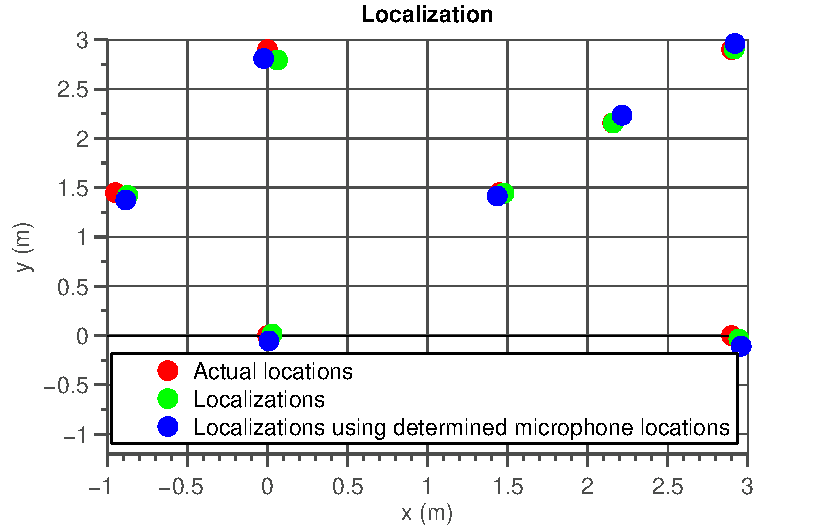
\includegraphics[width=.8\linewidth]{../../deliverable-7-resources/figures/ass-2/report-6/ass-2-report-6.pdf}
	\end{center}
	\caption{Localization using the TDOA data}
	\label{fig:ass-2-rep-6}
\end{figure}
Figure \ref{fig:ass-2-rep-6} shows the result of our localization algorithm on the TDOA data. Red dots indicate the actual positions of the beacon, while the green dots are the locations determined with our algorithm. By inspection the approximation seems quite alright, and the raw data confirms it is not too shabby with a mean error of \SI{4.92}{\centi\meter} and an error standard deviation of \SI{4.16}{\centi\meter}. However, we believe these results may be improved in the coming weeks. It turned out that the performance of a two-dimensional localization algorithm was better than the three-dimensional version as described in the manual \cite{epo4-manual}, so we decided to drop the z-axis. Reducing the problem to the two dimensional case makes the problem over-determined and allows us to -- in the coming weeks -- optimize the use of the additional information for example by iterative optimization methods. 

\subsection{Report 7}
\begin{figure}[H]
	\begin{subfigure}{.49\textwidth}
		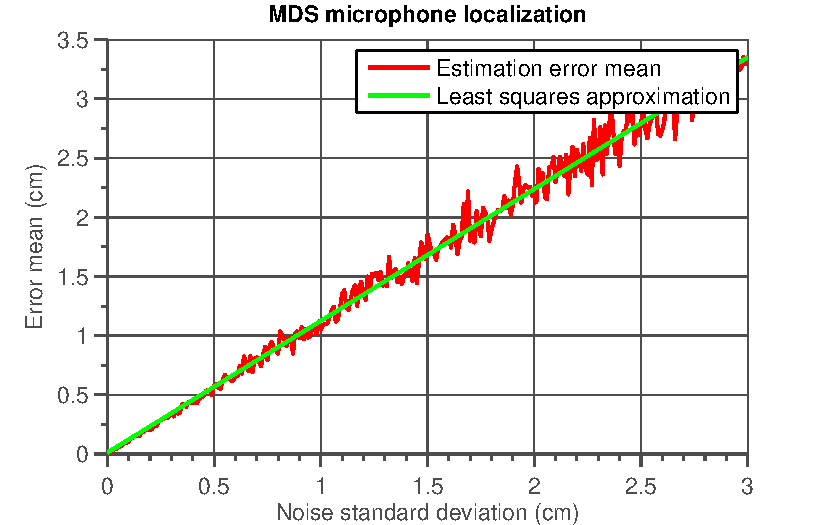
\includegraphics[width=\linewidth]{../../deliverable-7-resources/figures/ass-2/report-7-8/ass-2-report-7-mean.pdf}
		\caption{\centering Mean of the microphone localization error by the MDS algorithm}
	\end{subfigure}
	\begin{subfigure}{.49\textwidth}
		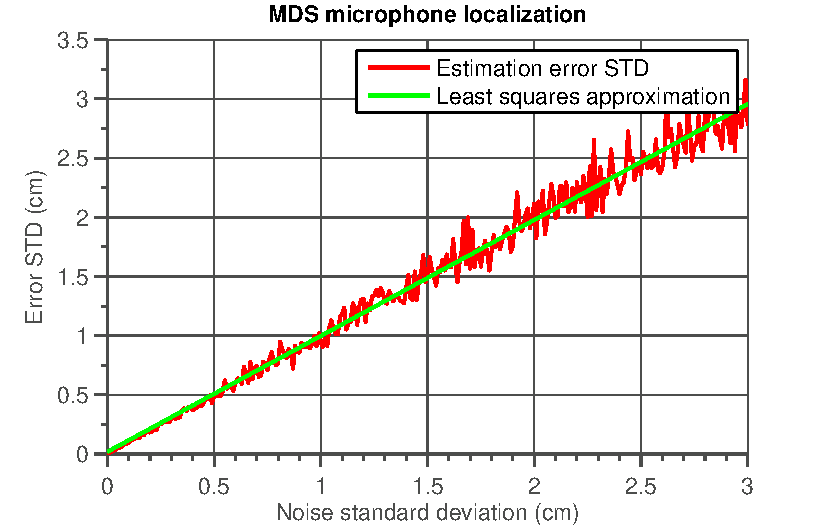
\includegraphics[width=\linewidth]{../../deliverable-7-resources/figures/ass-2/report-7-8/ass-2-report-7-std.pdf}
		\caption{\centering Standard deviation of the microphone localization error by the MDS algorithm}
	\end{subfigure}
	\caption{Mean and standard deviation of MDS microphone localization algorithm errors as a function of the standard deviation of noise, $\sigma$}
	\label{fig:ass-2-rep-7}
\end{figure}

Figure \ref{fig:ass-2-rep-7} shows the mean and standard deviation of the error of the MDS estimates for varying standard deviations of added noise. It is quite clear that a ordinary least squares approximation is quite a good fit. The resulting equations are:
\begin{align*}
\text{MDS localization error mean} = 1.11\cdot\sigma_{\text{noise}} \\
\text{MDS localization error standard deviation} = 0.98\cdot\sigma_{\text{noise}}
\end{align*}

Since we don't know what the noise levels during the final challenge will be and the performance of the MDS algorithm is not too good given noise, we expect that measuring the distances between the microphones by hand will produce a more accurate microphone map.
\subsection{Report 8}
Four microphones are indeed sufficient to determine their locations in the room in three dimensions. However, since the height of the car is constant and known and assuming the microphones are at the same, fixed height, the third dimension really plays no role and the fourth measurement can be used to improve the two dimensional model.

\subsection{Report 9}
\label{subsec:ass-2-rep-9}
\begin{figure}[H]
	\begin{center}
		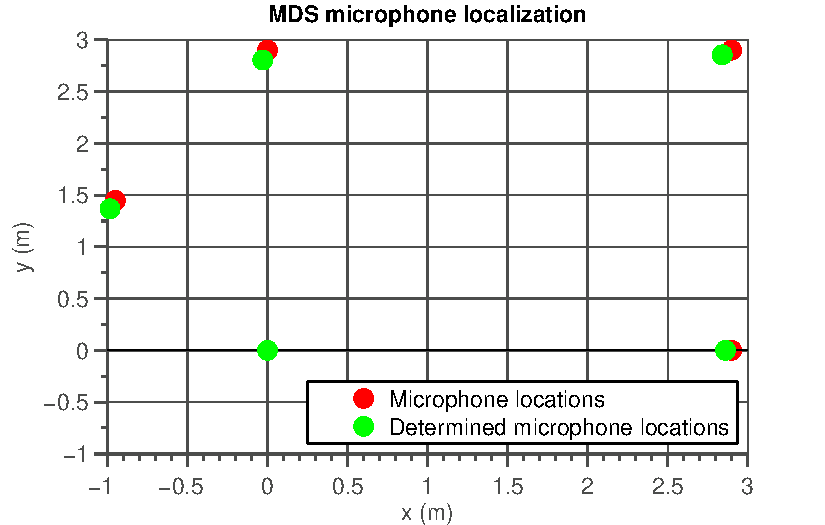
\includegraphics[width=.8\linewidth]{../../deliverable-7-resources/figures/ass-2/report-9/ass-2-report-9.pdf}
	\end{center}
	\caption{Microphone localization using the MDS algorithm}
	\label{fig:ass-2-rep-9}
\end{figure}
Figure~\ref{fig:ass-2-rep-9} shows the results of our microphone localization using the TDOA data, in which the mean positioning error is \SI{6.03}{\centi\meter} and the standard deviation of this error is \SI{4.08}{\centi\meter}. Of course, this estimate can be improved when the TDOA algorithm works better, i.e. making the trade-off between high required processing power and high sampling frequency tend more to the sampling frequency side. In its current state, the MDS algorithm could be used as a part of the KITT control system, but it might be better to tweak the algorithm and attempt to improve TDOA estimations before doing that.

\end{document}